\section{Bonus}
This section uses the variance Criterion to find the $\pi$ number. Here is the result of the $\pi$ estimation with different variances:
\newpage
\begin{itemize}
    \item $\sigma = 10^{-4}$, $\pi = 3.4435$
    \begin{figure}[H] 
     	\caption{$\sigma = 10^{-4}$ result} 
     	\centering 
     	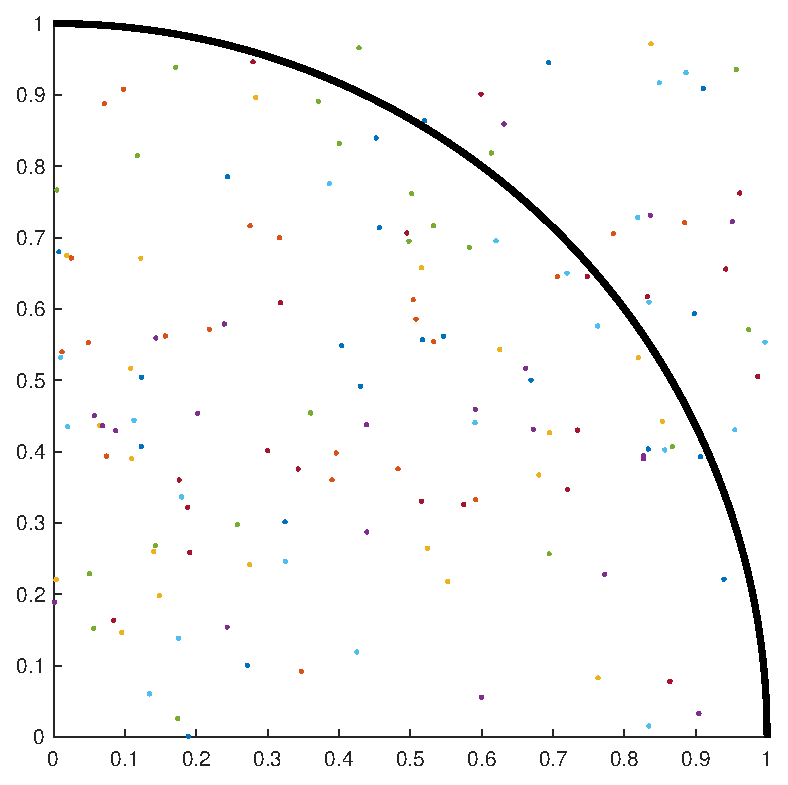
\includegraphics[width=9cm]{../Figure/Bonus/mont_e4} 
    \end{figure}
    \item $\sigma = 10^{-5}$, $\pi = 3.2188$
    \begin{figure}[H] 
        \caption{$\sigma = 10^{-5}$ result} 
        \centering 
        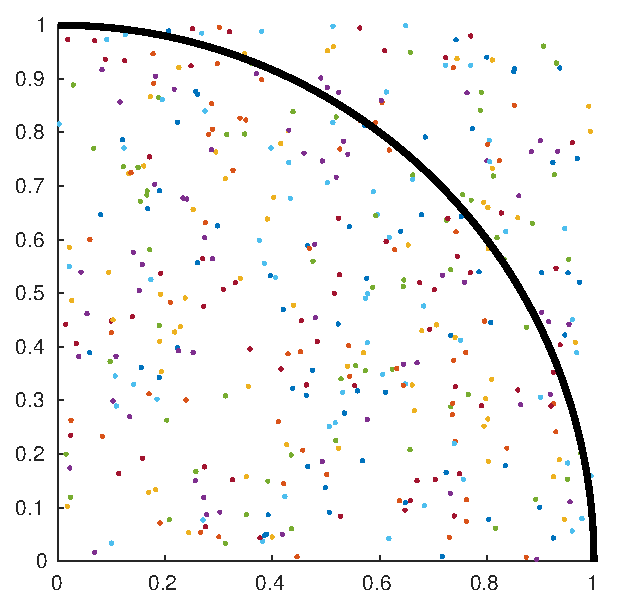
\includegraphics[width=9cm]{../Figure/Bonus/mont1e-05.eps} 
   \end{figure}
    \item $\sigma = 10^{-6}$, $\pi = 3.1379$
    \begin{figure}[H] 
        \caption{$\sigma = 10^{-6}$ result} 
        \centering 
        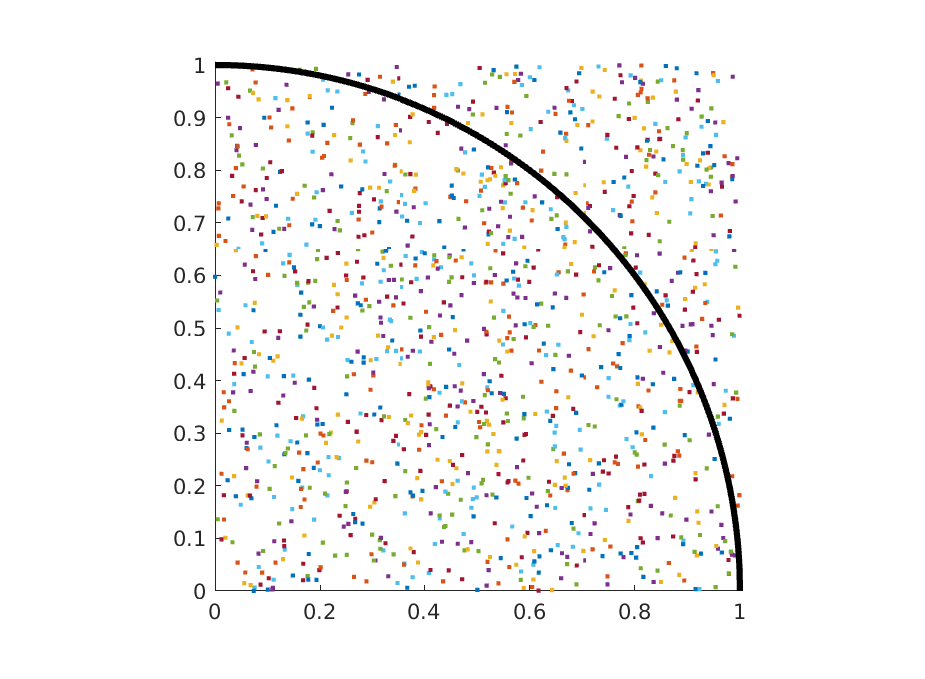
\includegraphics[width=12cm]{../Figure/Bonus/mont1e-06.eps} 
   \end{figure}
    \item $\sigma = 10^{-7}$, $\pi = 3.1589$
    \begin{figure}[H] 
        \caption{$\sigma = 10^{-7}$ result} 
        \centering 
        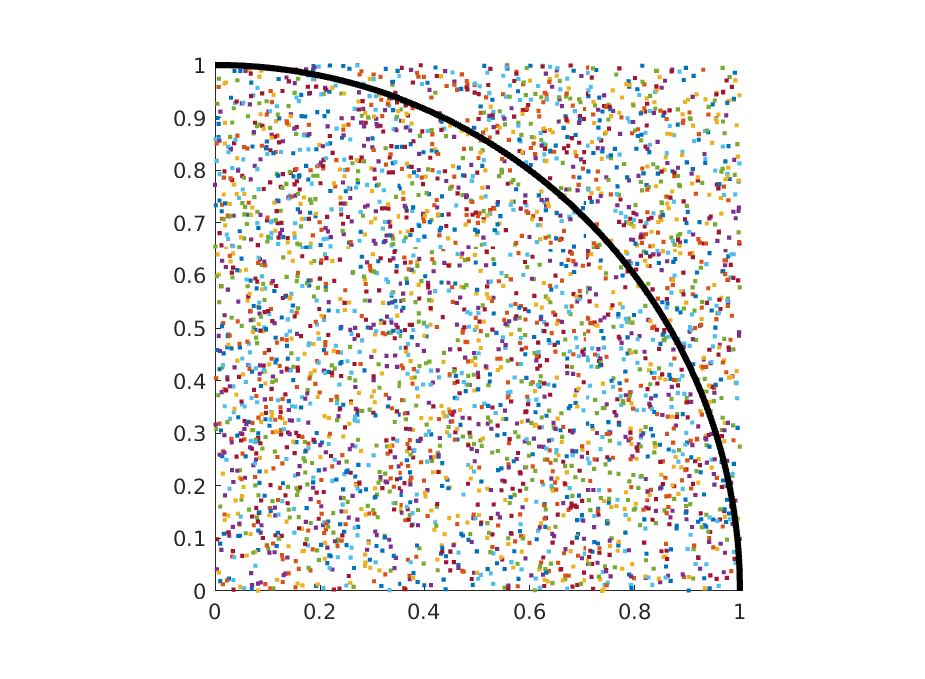
\includegraphics[width=12cm]{../Figure/Bonus/mont1e-07.eps} 
   \end{figure}
    \item $\sigma = 10^{-8}$, $\pi = 3.1120$
    \begin{figure}[H] 
        \caption{$\sigma = 10^{-8}$ result} 
        \centering 
        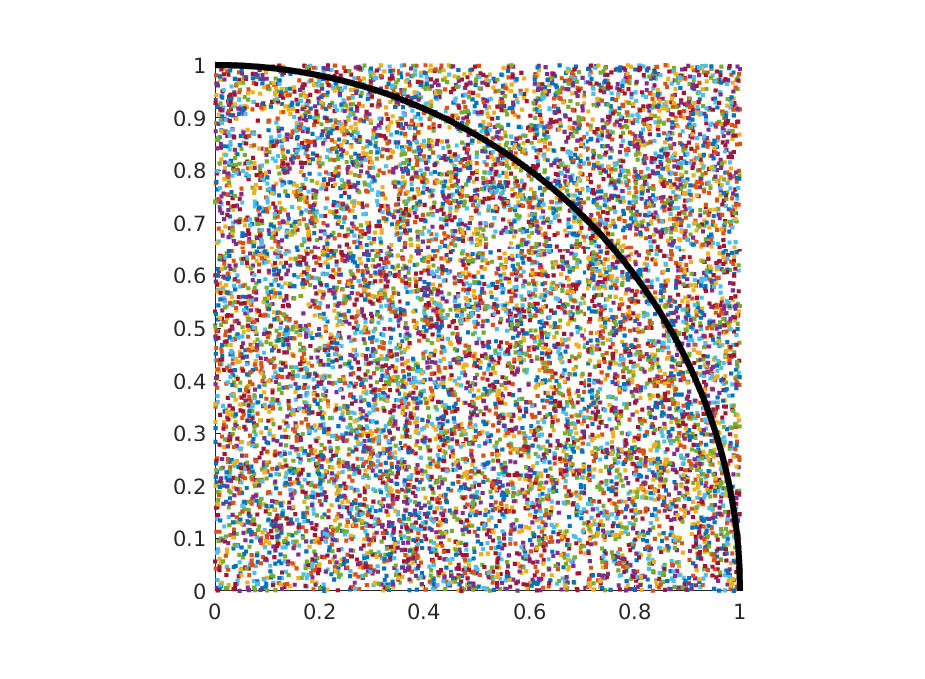
\includegraphics[width=12cm]{../Figure/Bonus/mont1e-08.eps} 
   \end{figure}
    \item $\sigma = 10^{-9}$, $\pi = 3.1441$
    \begin{figure}[H] 
        \caption{$\sigma = 10^{-9}$ result} 
        \centering 
        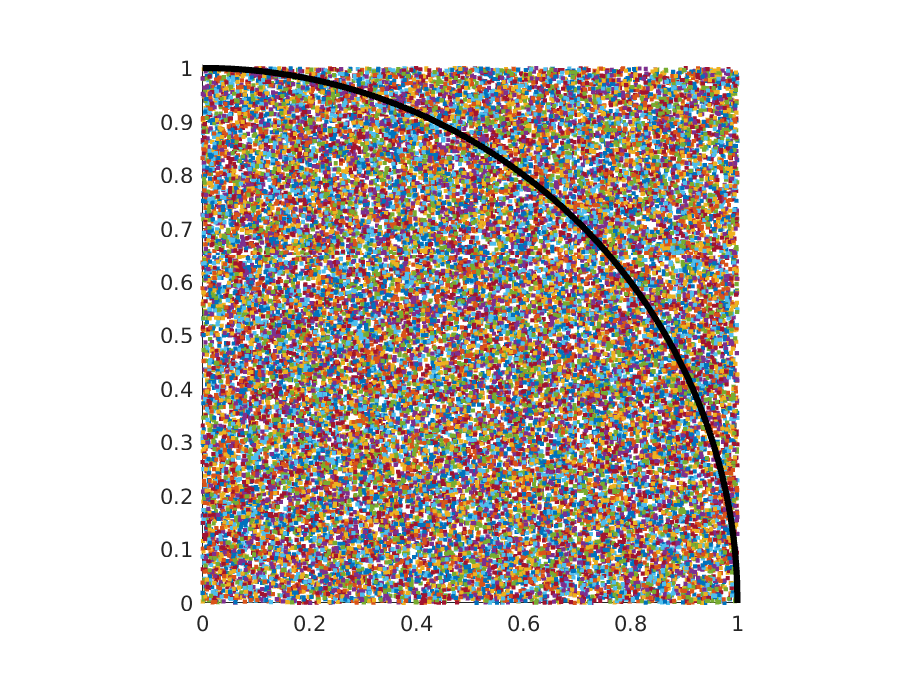
\includegraphics[width=12cm]{../Figure/Bonus/mont1e-09.eps} 
   \end{figure}
\end{itemize}

Here is plot of estimated $pi$ verses random number used in calculation.

    \begin{figure}[H] 
	\caption{$\pi$ estimation} 
	\centering 
	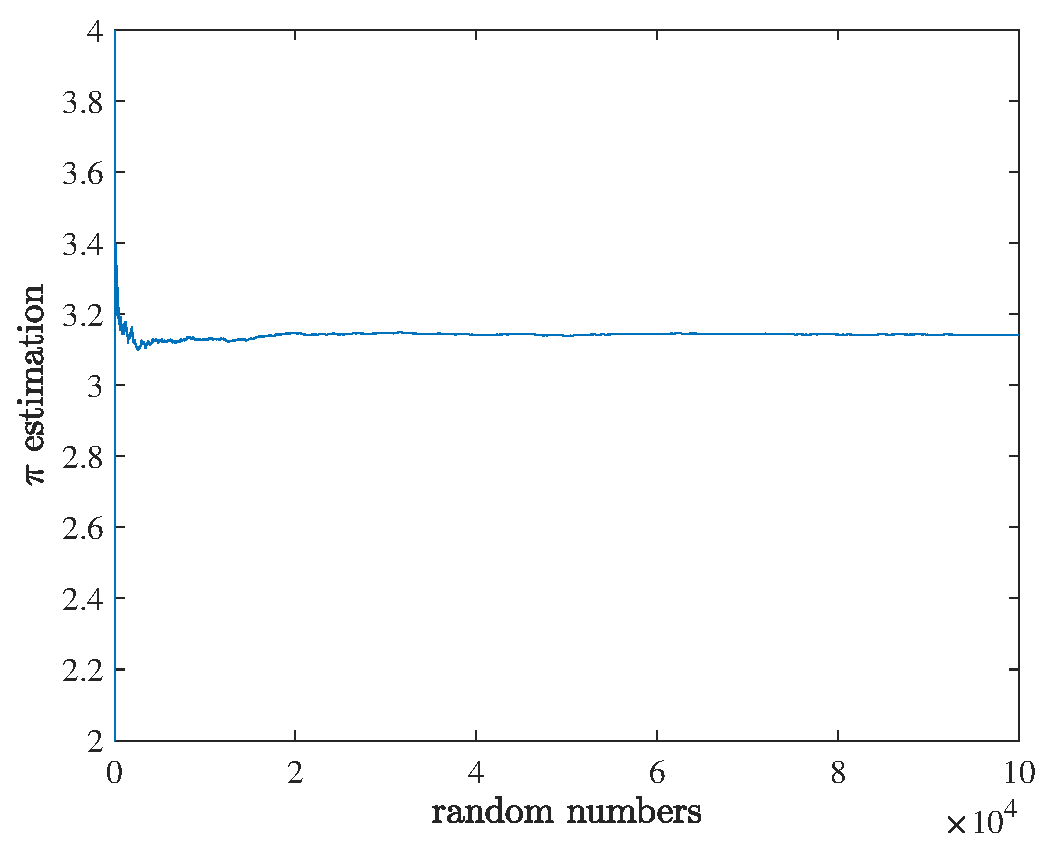
\includegraphics[width=12cm]{../Figure/Bonus/mont_pi} 
\end{figure}